% ----------------------------------------------------------------------------
%                             RESULTADOS
% ----------------------------------------------------------------------------
\chapter{Resultados}
\label{chap:Resultados E Interfaces Do Sistema}

Este capítulo apresenta os relatos do processo de desenvolvimento, as dificuldades, os desafios técnicos enfrentados e a descrição das interfaces codificadas que compõem o sistema TEia. Na tarefa de desenvolvimento do projeto, foi necessário um estudo aprofundado da manipulação nativa do \textit{Document Object Model} (DOM) utilizando \textit{Vanilla JS}, da separação de responsabilidades (\textit{Clean Code}) e da estruturação visual responsiva (\textit{Mobile-First}) através de CSS Grid e Flexbox.

Esses estudos permitiram afastar a complexidade excessiva (\textit{over-engineering}) inerente a \textit{frameworks} robustos (como ReactJS ou NextJS) em prol de uma aplicação leve, ágil e focada na baixa carga cognitiva. A decisão por tecnologias web puras garantiu total autonomia sobre a arquitetura e facilitou a adaptação direta das regras de negócio.

A seguir, será demonstrado como se deu o desafio de integrar a manipulação de estados via \textit{localStorage} e as lógicas de acesso condicional às interfaces, garantindo que os requisitos funcionais delineados no capítulo anterior fossem traduzidos em fluxos visuais que efetivamente suportam o manejo comportamental de alunos com TDAH e TOD.

\vspace{0.5cm}
\section{Retrospectiva e Desafios}

A partir do planejamento do projeto, detalhado no cronograma apresentado na Seção 4.1, foi realizado um rigoroso levantamento de requisitos de usuário, funcionais e não funcionais. Essa etapa possibilitou uma compreensão profunda do cenário educacional e direcionou a proposta de desenvolvimento do sistema TEia. As fases de análise de projeto permitiram o entendimento e a criação do diagrama de casos de uso macro do sistema. Posteriormente, as telas da aplicação foram prototipadas em alta fidelidade no Figma para o enriquecimento visual e a validação dos requisitos levantados, propiciando um amadurecimento da visão do usuário sobre a interação com a plataforma.

Ao iniciar a etapa de estudos das tecnologias elencadas para o desenvolvimento, o projeto deparou-se com o desafio da escolha arquitetônica. Inicialmente, havia a intenção de utilizar bibliotecas baseadas em componentes, como o React.js. Contudo, direcionando esforços para a compreensão da infraestrutura escolar e do perfil dos utilizadores, identificou-se a oportunidade e a necessidade de adotar o JavaScript puro (\textit{Vanilla JS}). Essa decisão exigiu a superação de desafios técnicos ligados à manipulação nativa do \textit{Document Object Model} (DOM) e à manutenção de um código modular e limpo (\textit{Clean Code}), permitindo uma melhor adequação, leveza e alta performance nos computadores institucionais.

O desenvolvimento da solução exigiu intenso esforço e dedicação, em virtude do desafio de codificar as principais funcionalidades do sistema a partir do zero. Destacam-se, nesse processo, a implementação do motor de busca com filtros combinados instantâneos operando diretamente no lado do cliente, a integração do \textit{back-end} via Firebase para a sincronização em tempo real da linha do tempo (\textit{timeline}) familiar, e a estruturação lógica para a geração automatizada de relatórios em PDF.

A estratégia de implementação da solução baseada em uma Arquitetura Web Responsiva, com \textit{design Mobile-First}, permitiu agregar ao projeto a flexibilidade necessária. Essa abordagem garantiu o acesso ágil tanto pelo navegador \textit{web} (computador do educador na escola) quanto pelo dispositivo móvel (pais acompanhando a rotina em casa), contornando a resistência inicial dos docentes em efetuar \textit{downloads} ou usar pacotes de dados pessoais, e adaptando o comportamento da aplicação perfeitamente a qualquer ecrã. Nas subseções a seguir, serão apresentados os resultados das interfaces de interação do projeto, bem como a explanação das funcionalidades implementadas.

\vspace{0.5cm}
\section{Interfaces do Sistema}

Esta seção apresenta as capturas de tela (\textit{screenshots}) das interfaces finais codificadas para a aplicação web TEia. O \textit{design} implementado reflete a arquitetura \textit{Mobile-First}, evidenciando a responsividade nativa construída com HTML5 e CSS3, que permite a adaptação visual fluida tanto para \textit{desktops} (computadores institucionais) quanto para \textit{smartphones} (dispositivos móveis das famílias).

\vspace{0.5cm}
\section{Autenticação e Controle de Acesso \textit{(Login)}}

A Figura 5.1 apresenta a tela de (\textit{login}) da plataforma. Nesta tela, o usuário é recebido por uma interface minimalista e acolhedora, cujo objetivo é reduzir a carga cognitiva desde o primeiro contato. O destaque central da interface é a seleção do perfil de acesso, permitindo que o usuário identifique-se de forma clara antes da inserção das credenciais.

A segregação inicial não é apenas um recurso visual, mas o gatilho para as regras de negócio estruturadas no \textit{back-end} via \textit{Firebase Authentication}. Ao selecionar o perfil de "Educador", o sistema aciona uma validação rigorosa, bloqueando tentativas de acesso com e-mails genéricos e exigindo, obrigatoriamente, o uso do domínio institucional da escola (\texttt{@ifb.edu.br}). Abaixo dos botões de perfil, encontram-se os campos padronizados para a inserção de e-mail e senha, atalhos para recuperação de acesso e a opção de novo cadastro.

\begin{figure}[H]
  \centering
  \caption{Tela de \textit{login}}
  \label{fig:tela_login}
  \vspace{0.3cm}

  \begin{minipage}[b]{0.77\textwidth}
    \centering
    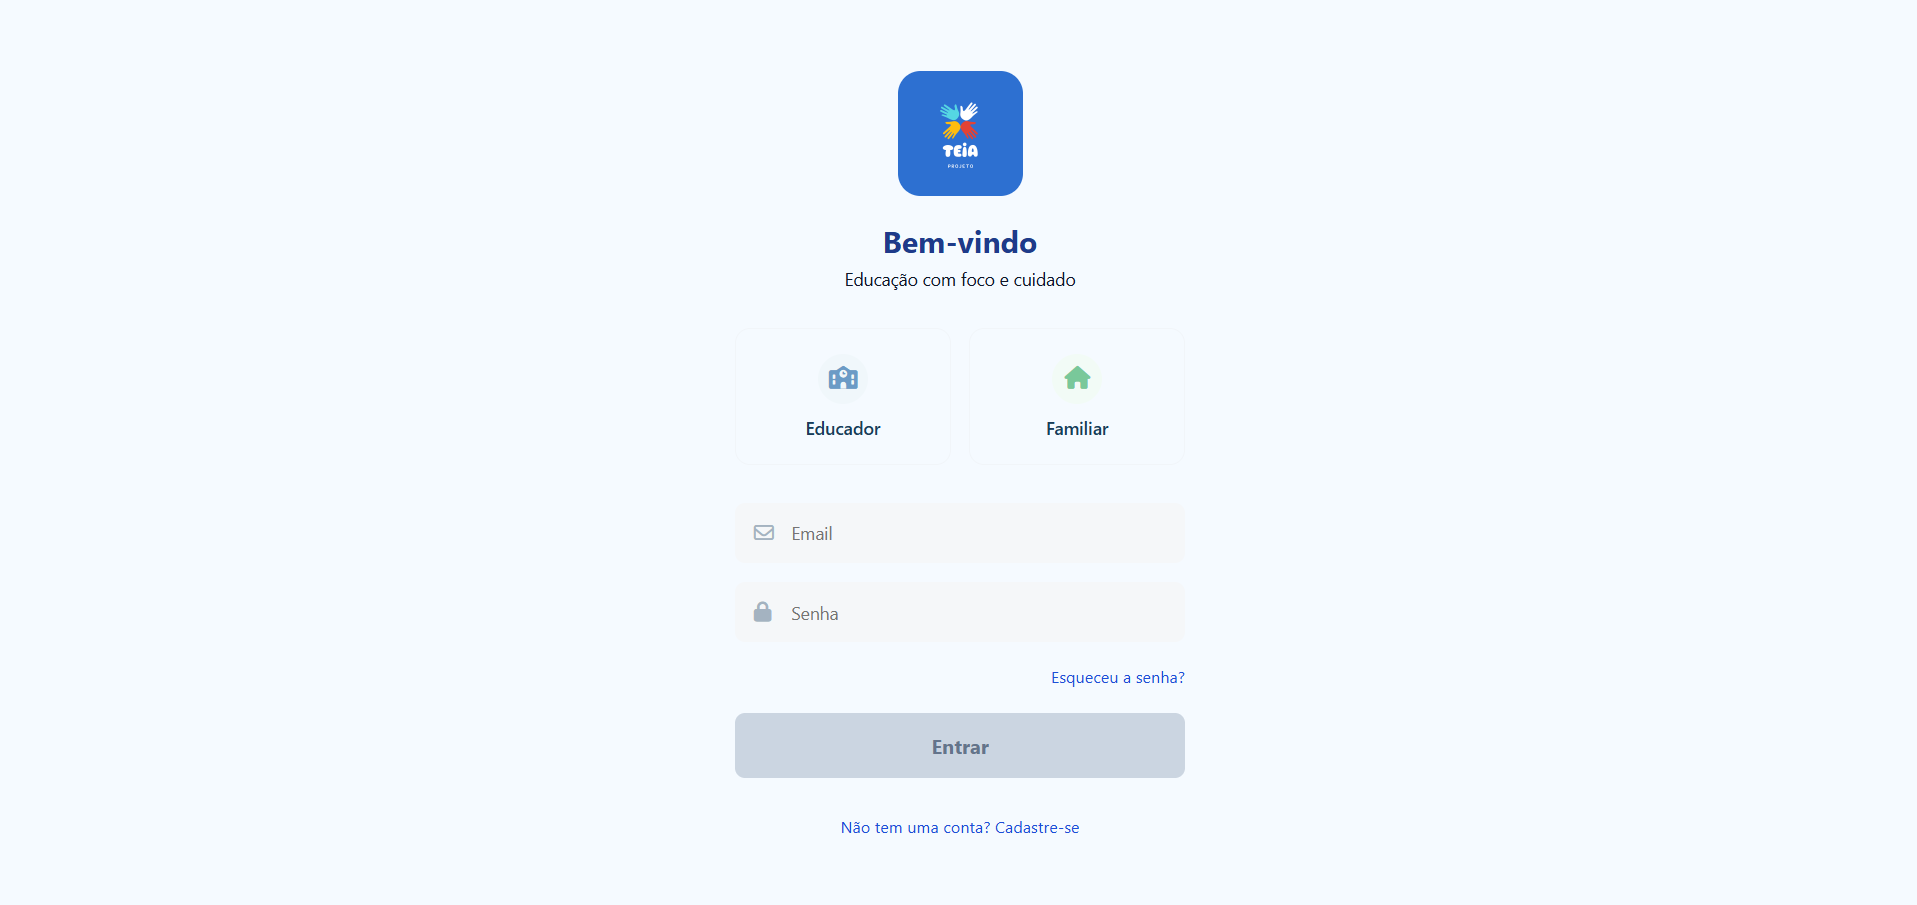
\includegraphics[width=\textwidth, keepaspectratio]
    {assets/telaLogin_desktop}
    \vspace{0.1cm}
    \centerline{\small (a) Desktop} % <-- Subtítulo A
  \end{minipage}\hfill
  \begin{minipage}[b]{0.22\textwidth}
    \centering
    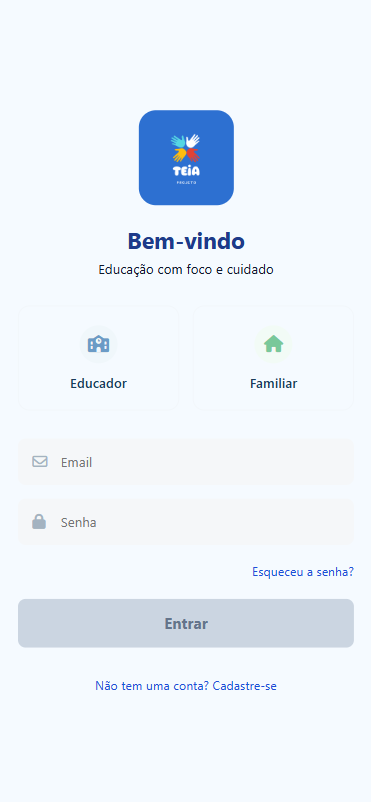
\includegraphics[width=\textwidth, keepaspectratio]
    {assets/telaLogin_mobile}
    \vspace{0.1cm}
        \centerline{\small (b) Mobile}
  \end{minipage}

  \vspace{0.3cm}
  \begin{flushleft}
  \footnotesize{Fonte: Elaborada pela autora (2026).}
  \end{flushleft}
\end{figure}

\vspace{0.5cm}
\section{Interfaces do Perfil Educador}

O perfil Educador é o núcleo de alimentação de dados do sistema TEia. As interfaces a seguir foram concebidas para garantir extrema agilidade no manejo de rotinas e crises em sala de aula.

\vspace{0.5cm}
\subsection{Cadastrar Nova Turma}

A Figura 5.2 apresenta a interface dedicada ao cadastro e gestão de novas turmas ("Cadastrar Nova Turma"). Esta tela é o ponto de partida operacional para o educador no sistema TEia após a autenticação. A interface utiliza um formulário de campo único e direto, minimizando a fricção no registro de informações.

Ao inserir o nome da turma e clicar no botão de ação primária "Salvar Turma", a lógica implementada em \textit{Vanilla JS} processa a entrada e atualiza a listagem logo abaixo. A área "Turmas Cadastradas" apresenta um painel vertical limpo, onde cada turma salva (ex: "1º Ano A - Matutino") é exibida em \textit{cards} padronizados. Este fluxo garante que a estruturação do ambiente letivo virtual seja feita de forma rápida, delegando a persistência desses dados diretamente ao \textit{localStorage} na versão inicial e, posteriormente, ao banco de dados \textit{Firestore}.

\begin{figure}[H]
  \centering
  \caption{Tela de cadastrar nova turma}
  \label{fig:tela_cadastrarNovaTurma}
  \vspace{0.3cm}

  \begin{minipage}[b]{0.77\textwidth}
    \centering
    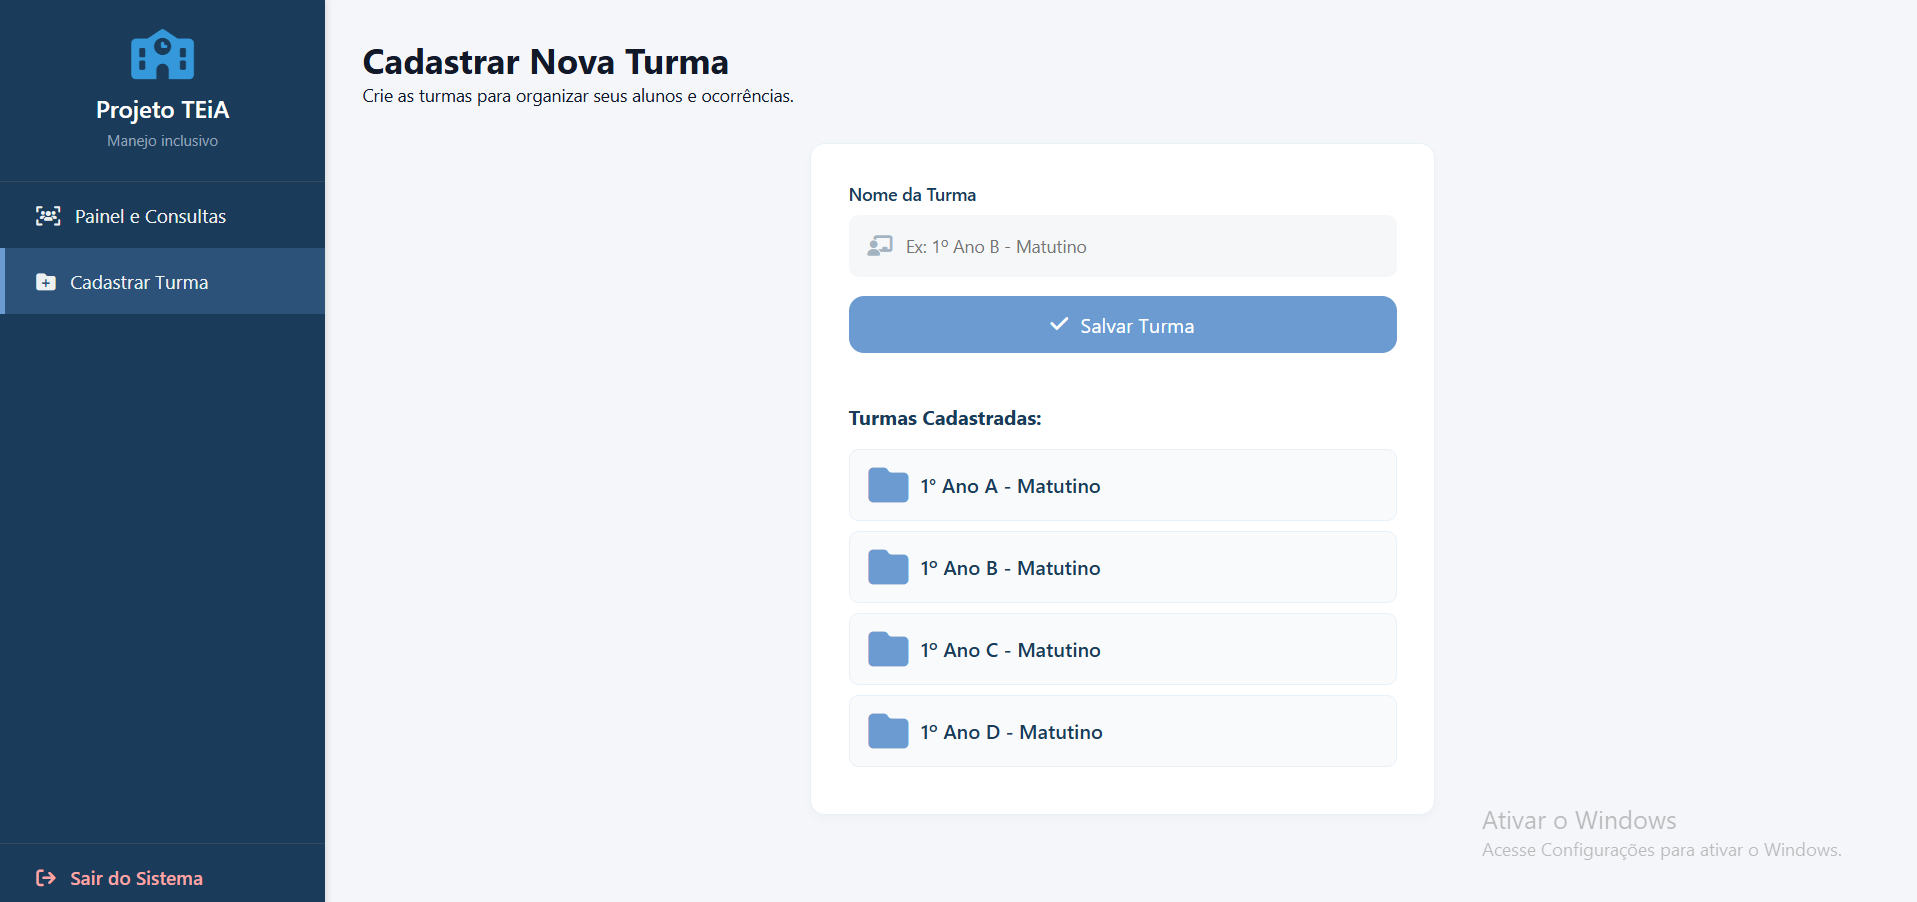
\includegraphics[width=\textwidth, keepaspectratio]
    {assets/CadastrarNovaTurma_desktop}
    \vspace{0.1cm}
    \centerline{\small (a) Desktop} % <-- Subtítulo A
  \end{minipage}\hfill
  \begin{minipage}[b]{0.22\textwidth}
    \centering
    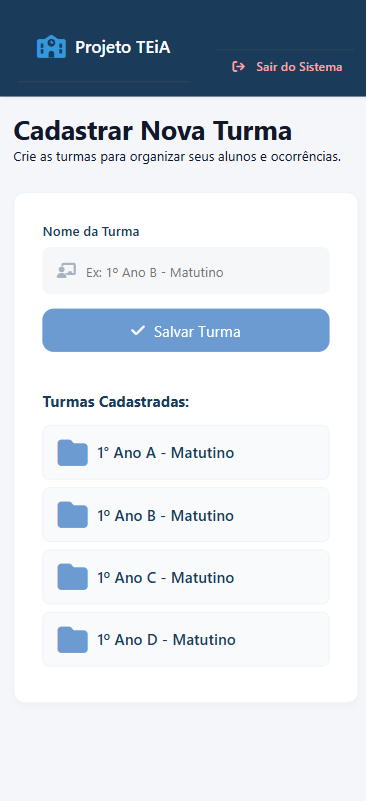
\includegraphics[width=\textwidth, keepaspectratio]
    {assets/CadastrarNovaTurma_mobile}
    \vspace{0.1cm}
        \centerline{\small (b) Mobile}
  \end{minipage}

  \vspace{0.3cm}
  \begin{flushleft}
  \footnotesize{Fonte: Elaborada pela autora (2026).}
  \end{flushleft}
\end{figure}

\vspace{0.5cm}
\subsection{Matricular Novo Aluno}

A Figura 5.3 apresenta o formulário "Matricular Novo Estudante", acionado pelo educador para povoar as suas turmas no sistema. Este fluxo foi concebido com uma interface fluida, onde a entrada de dados se resume a informações estritamente necessárias, alinhando-se aos princípios da baixa carga cognitiva exigida na rotina escolar.

O \textit{design} do formulário inclui ícones indicativos nos campos de texto, facilitando o reconhecimento instantâneo da informação solicitada. O educador preenche o "Nome Completo do Estudante" e tem à disposição campos de recolha de dados fundamentais para a arquitetura do sistema TEia: a matrícula institucional, a indicação clínica de Neurodivergência/Condição (ex: TDAH, TOD, TEA) e o e-mail do familiar responsável. 

A inclusão do e-mail do familiar, assinalado como opcional no formulário, atua como o principal gatilho do sistema: é ele que cria a ponte de comunicação com o ambiente doméstico, permitindo que a aplicação relacione este aluno específico ao futuro painel de acesso dos pais. Ao clicar em "Salvar Cadastro", o código processa a validação dos campos no lado do cliente (\textit{client-side}) e vincula automaticamente o perfil do estudante à turma previamente selecionada pelo professor.

\begin{figure}[H]
  \centering
  \caption{Tela de matricular novo estudante}
  \label{fig:tela_novoAluno}
  \vspace{0.3cm}

  \begin{minipage}[b]{0.77\textwidth}
    \centering
    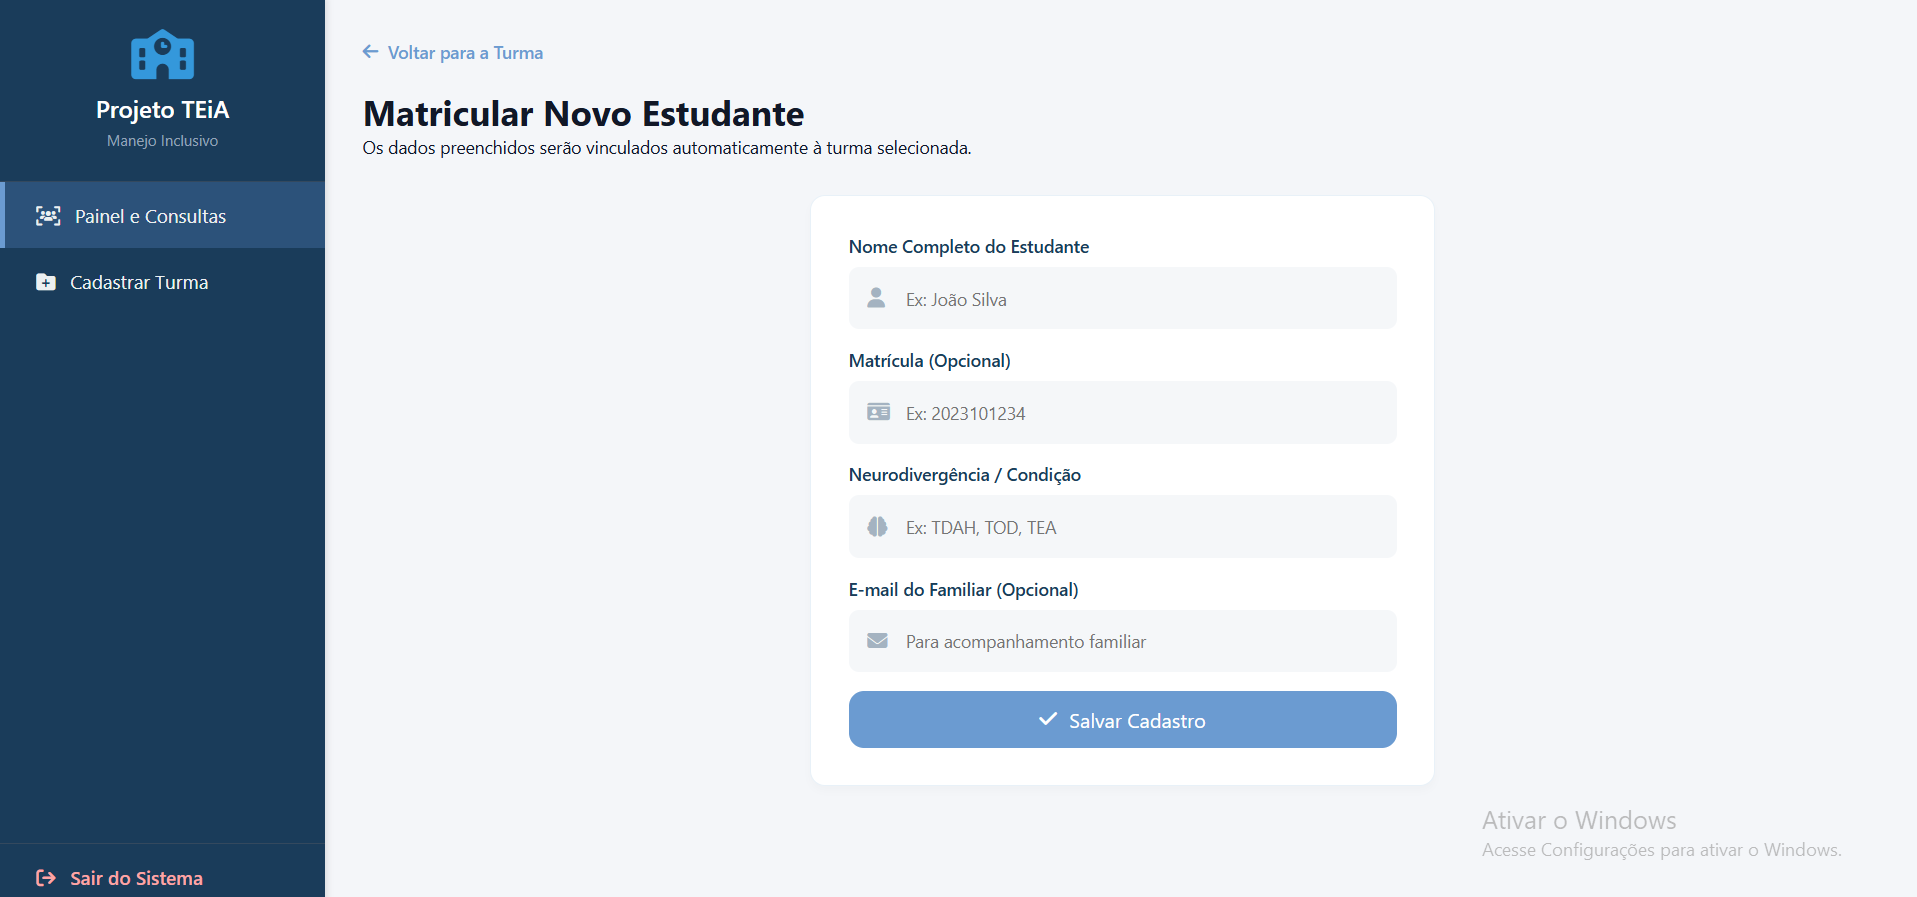
\includegraphics[width=\textwidth, keepaspectratio]
    {assets/novoAluno_desktop}
    \vspace{0.1cm}
    \centerline{\small (a) Desktop} % <-- Subtítulo A
  \end{minipage}\hfill
  \begin{minipage}[b]{0.22\textwidth}
    \centering
    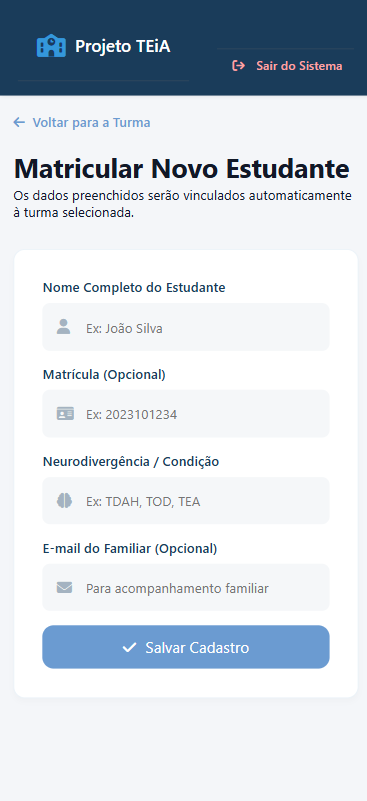
\includegraphics[width=\textwidth, keepaspectratio]
    {assets/novoAluno_mobile}
    \vspace{0.1cm}
        \centerline{\small (b) Mobile}
  \end{minipage}

  \vspace{0.3cm}
  \begin{flushleft}
  \footnotesize{Fonte: Elaborada pela autora (2026).}
  \end{flushleft}
\end{figure}

\vspace{0.5cm}
\subsection{Painel de Consultas}

Após a etapa de cadastro inicial, o primeiro ambiente de gestão que o educador acessa é o "Painel de Turmas". Esta interface, ilustrada na Figura 5.4, funciona como o diretório principal do professor. A área central exibe as "Turmas Cadastradas" organizadas em \textit{cards} horizontais, acompanhadas de ícones em formato de pasta, o que remete intuitivamente à organização de arquivos e facilita o reconhecimento cognitivo.

O \textit{design} limpo desta interface permite que o docente visualize rapidamente todas as turmas sob a sua responsabilidade e clique na sala desejada para iniciar o manejo diário. No painel lateral fixo (à esquerda na versão \textit{desktop}), o usuário mantém acesso constante aos atalhos de "Painel e Consultas", "Cadastrar Turma" e à opção de segurança "Sair do Sistema". Na versão para dispositivos móveis, este menu lateral é condensado, garantindo a adaptação fluida ditada pela arquitetura \textit{Mobile-First}.

\begin{figure}[H]
    \centering
    \caption{Tela de painel de consultas}
    \label{fig:painelConsulta}
    
    \vspace{0.2cm}
    
   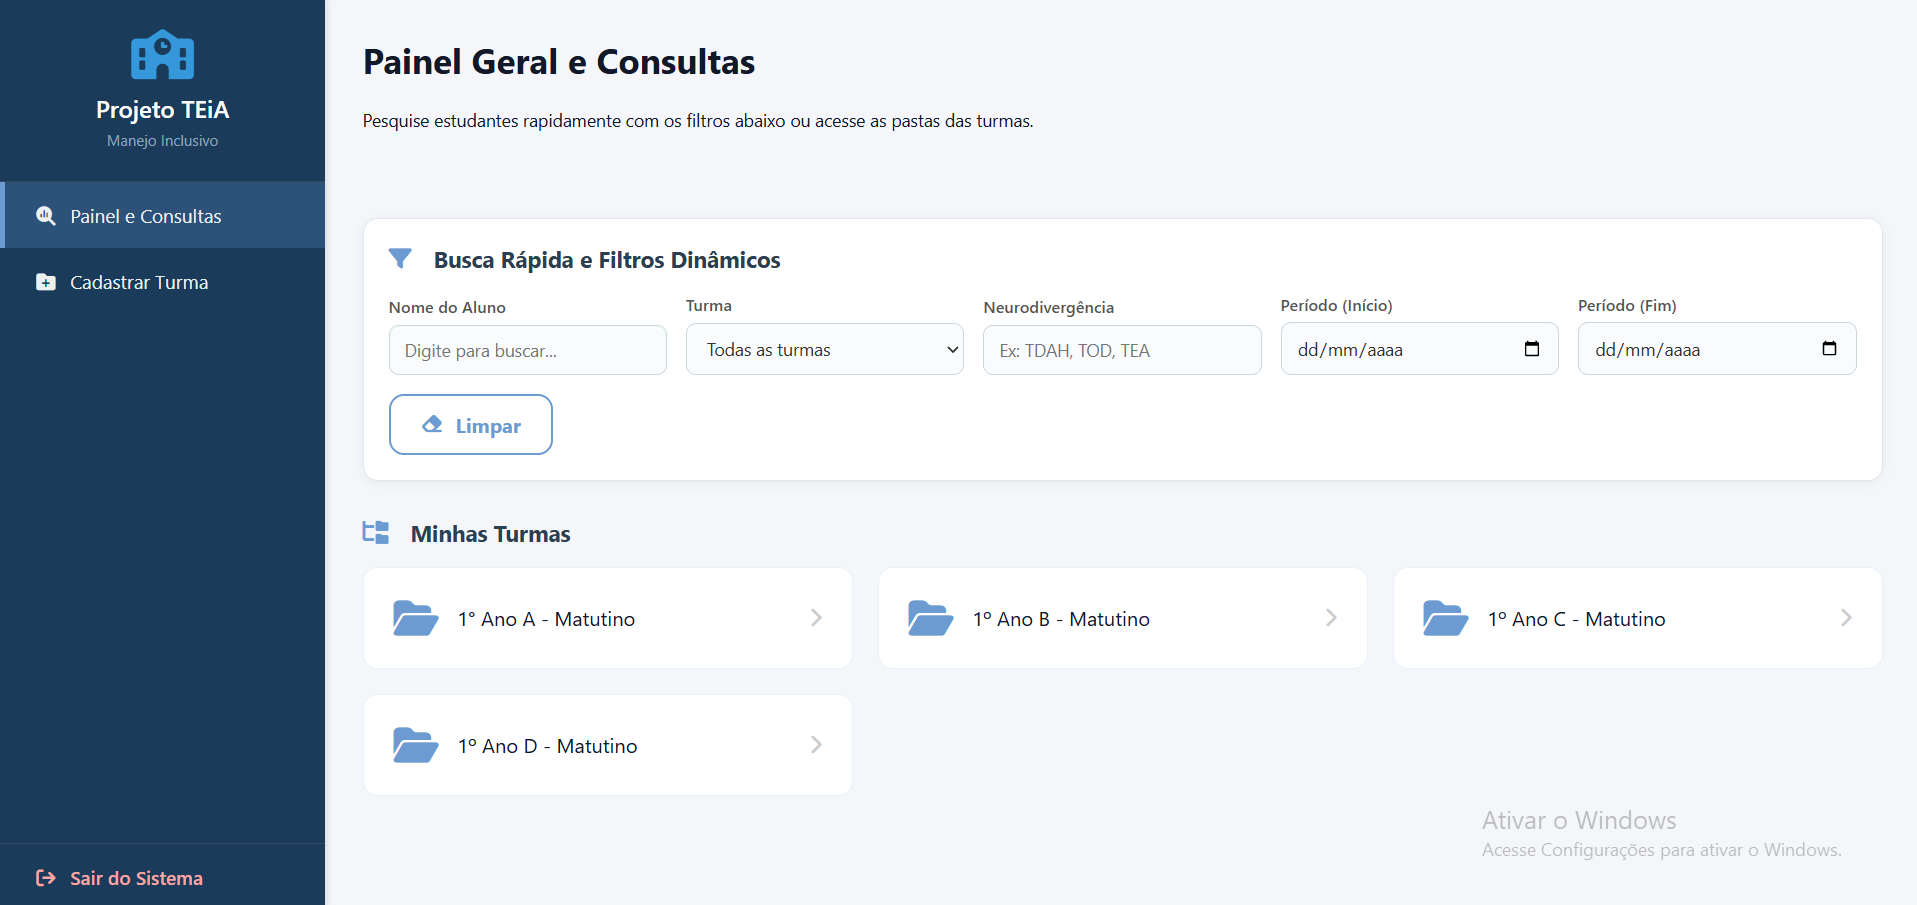
\includegraphics[width=0.8\textwidth, keepaspectratio]{assets/painelConsultas_desktop}
\end{figure}

\begin{figure}[H]
  \centering
  \vspace{0.3cm}

\centering % Centraliza o bloco das duas imagens na página
  \begin{minipage}[b]{0.22\textwidth}
    \centering
    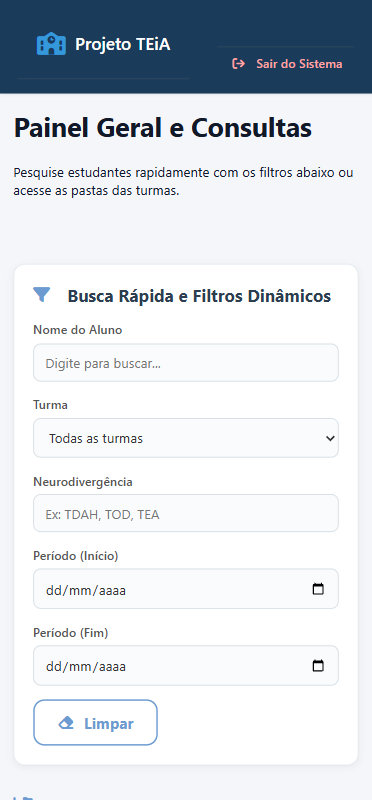
\includegraphics[width=\textwidth, keepaspectratio]{assets/painelConsultas_mobile1}
    \vspace{0.1cm}
    \centerline{\small (b) Mobile 1}
  \end{minipage}%
  \hspace{1cm} % <--- AJUSTE AQUI: Aumente ou diminua o valor (ex: 0.5cm, 2cm)
  \begin{minipage}[b]{0.22\textwidth}
    \centering
    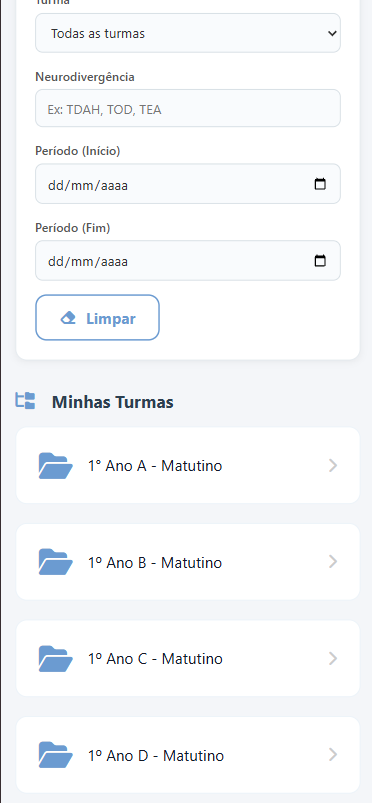
\includegraphics[width=\textwidth, keepaspectratio]{assets/painelConsultas_mobile2}
    \vspace{0.1cm}
    \centerline{\small (c) Mobile 2}
  \end{minipage}

  \vspace{0.3cm}
  \begin{flushleft}
  \footnotesize{Fonte: Elaborada pela autora (2026).}
  \end{flushleft}
\end{figure}

\vspace{0.5cm}
\subsection{Visão da Turma}

Ao selecionar uma classe específica no painel anterior, o educador é direcionado para a "Visão da Turma", ilustrada na Figura 5.5. A tela apresenta o nome da turma selecionada em destaque no cabeçalho (ex: "1º Ano A - Matutino") e disponibiliza a listagem interativa de todos os estudantes matriculados naquela classe.

A arquitetura visual desta tela foi desenhada para promover o acompanhamento rápido do \textit{status} comportamental do estudante. Isso é alcançado por meio de uma marcação colorida suave no \textit{card} do aluno (como o círculo verde demonstrado na imagem), que sinaliza ao educador a estabilidade ou a necessidade de atenção àquele perfil. Na própria listagem, a interface exibe o nome do estudante acompanhado das \textit{tags} de diagnóstico cadastradas (como "TEA e TDAH"), eliminando a necessidade de navegação profunda para a obtenção de dados básicos. 

Adicionalmente, a tela oferece comandos primários de administração da sala de aula, como "Excluir Turma" (em cor de alerta) e "Novo Aluno" (em azul, para ações construtivas), posicionados no canto superior direito, garantindo que as ferramentas de gestão estejam acessíveis sem poluir a área principal de leitura.

\begin{figure}[H]
  \centering
  \caption{Visão da Turma}
  \label{fig:tela_VisãoTurma}
  \vspace{0.3cm}

  \begin{minipage}[b]{0.77\textwidth}
    \centering
    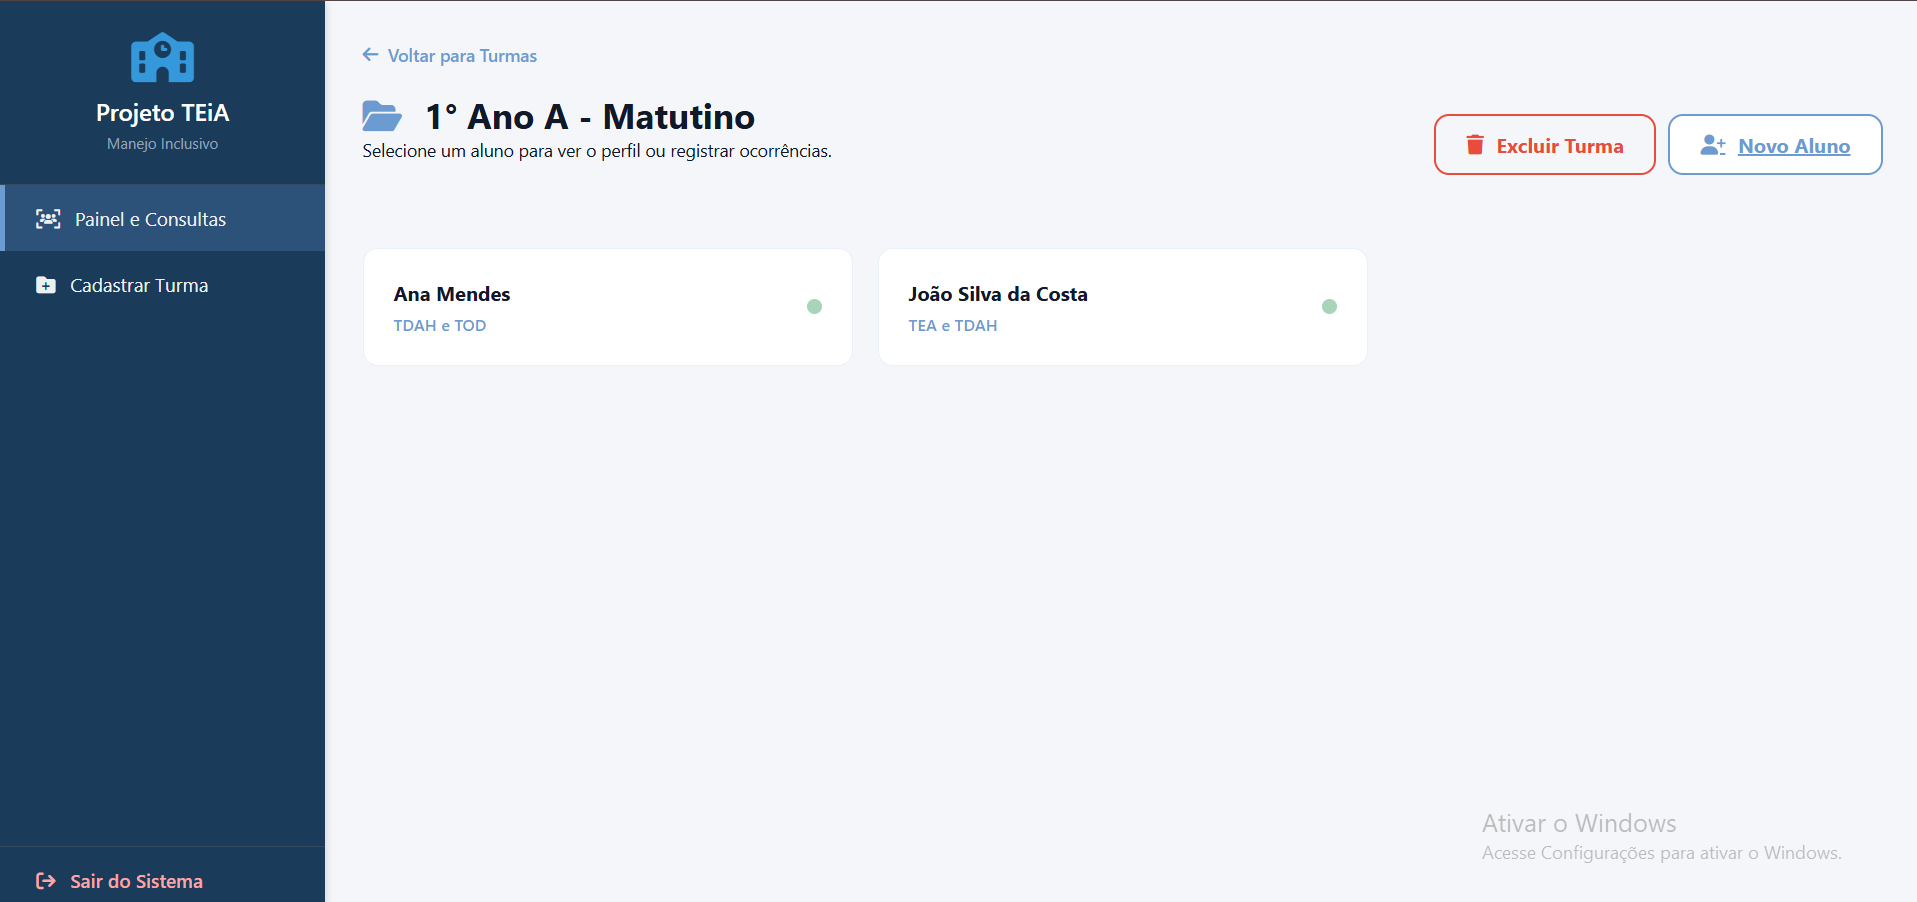
\includegraphics[width=\textwidth, keepaspectratio]
    {assets/visaoTurma_desktop}
    \vspace{0.1cm}
    \centerline{\small (a) Desktop} % <-- Subtítulo A
  \end{minipage}\hfill
  \begin{minipage}[b]{0.22\textwidth}
    \centering
    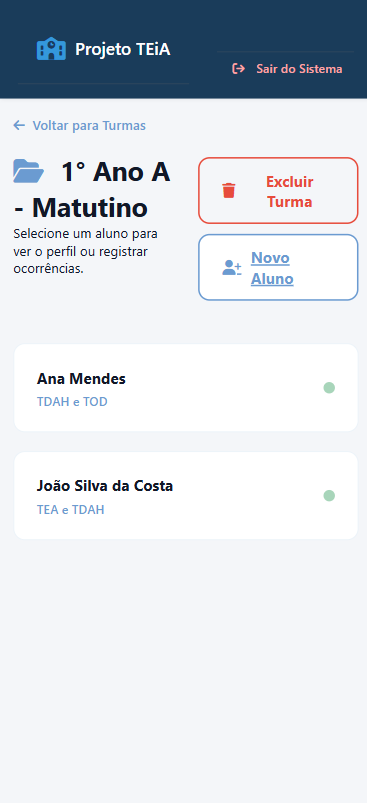
\includegraphics[width=\textwidth, keepaspectratio]
    {assets/visaoTurma_mobile}
    \vspace{0.1cm}
        \centerline{\small (b) Mobile}
  \end{minipage}

  \vspace{0.3cm}
  \begin{flushleft}
  \footnotesize{Fonte: Elaborada pela autora (2026).}
  \end{flushleft}
\end{figure}

\vspace{0.5cm}
\subsection{Perfil do Aluno}

A Figura 5.6 detalha a interface do perfil individual do aluno, que é acessada diretamente pelo educador ao clicar no \textit{card} do estudante no painel da turma. O cabeçalho desta página foca em apresentar o contexto clínico e administrativo de forma imediata: exibe o nome do estudante em destaque, o seu número de matrícula e as \textit{tags} de diagnóstico (ex: "TEA e TDAH"). Essa disposição garante que o professor tenha ciência das necessidades singulares da criança no primeiro segundo de leitura.

O corpo central da interface é preenchido pelo "Histórico Recente", uma linha do tempo (\textit{timeline}) vertical que lista cronologicamente as ocorrências documentadas. Cada evento registrado exibe a hora, a data, a descrição combinada dos comportamentos observados (ex: Agitação, Desatenção, Conflito, Impulsividade, Desafio), o nível de intensidade do evento (sinalizado de forma semântica com o uso das cores amarelo para "Leve", laranja para "Moderada" e vermelho para "Alta") e, caso existam, as notas em texto livre redigidas pelo professor, que aparecem formatadas em estilo de citação.

No topo direito da área do aluno encontram-se as opções de ação cruciais para o acompanhamento educacional. Destaca-se o botão de ação primária "Registrar Ocorrência", acompanhado das funcionalidades secundárias "Gerar Relatório" (voltado ao suporte clínico), "Mudar de Turma" e "Excluir Aluno", centralizando o controle operacional da trajetória do estudante na mesma tela em que o professor analisa a sua evolução diária.

\begin{figure}[H]
  \centering
  \caption{Perfil do aluno}
  \label{fig:tela_PerfilAluno}
  \vspace{0.3cm}

  \begin{minipage}[b]{0.77\textwidth}
    \centering
    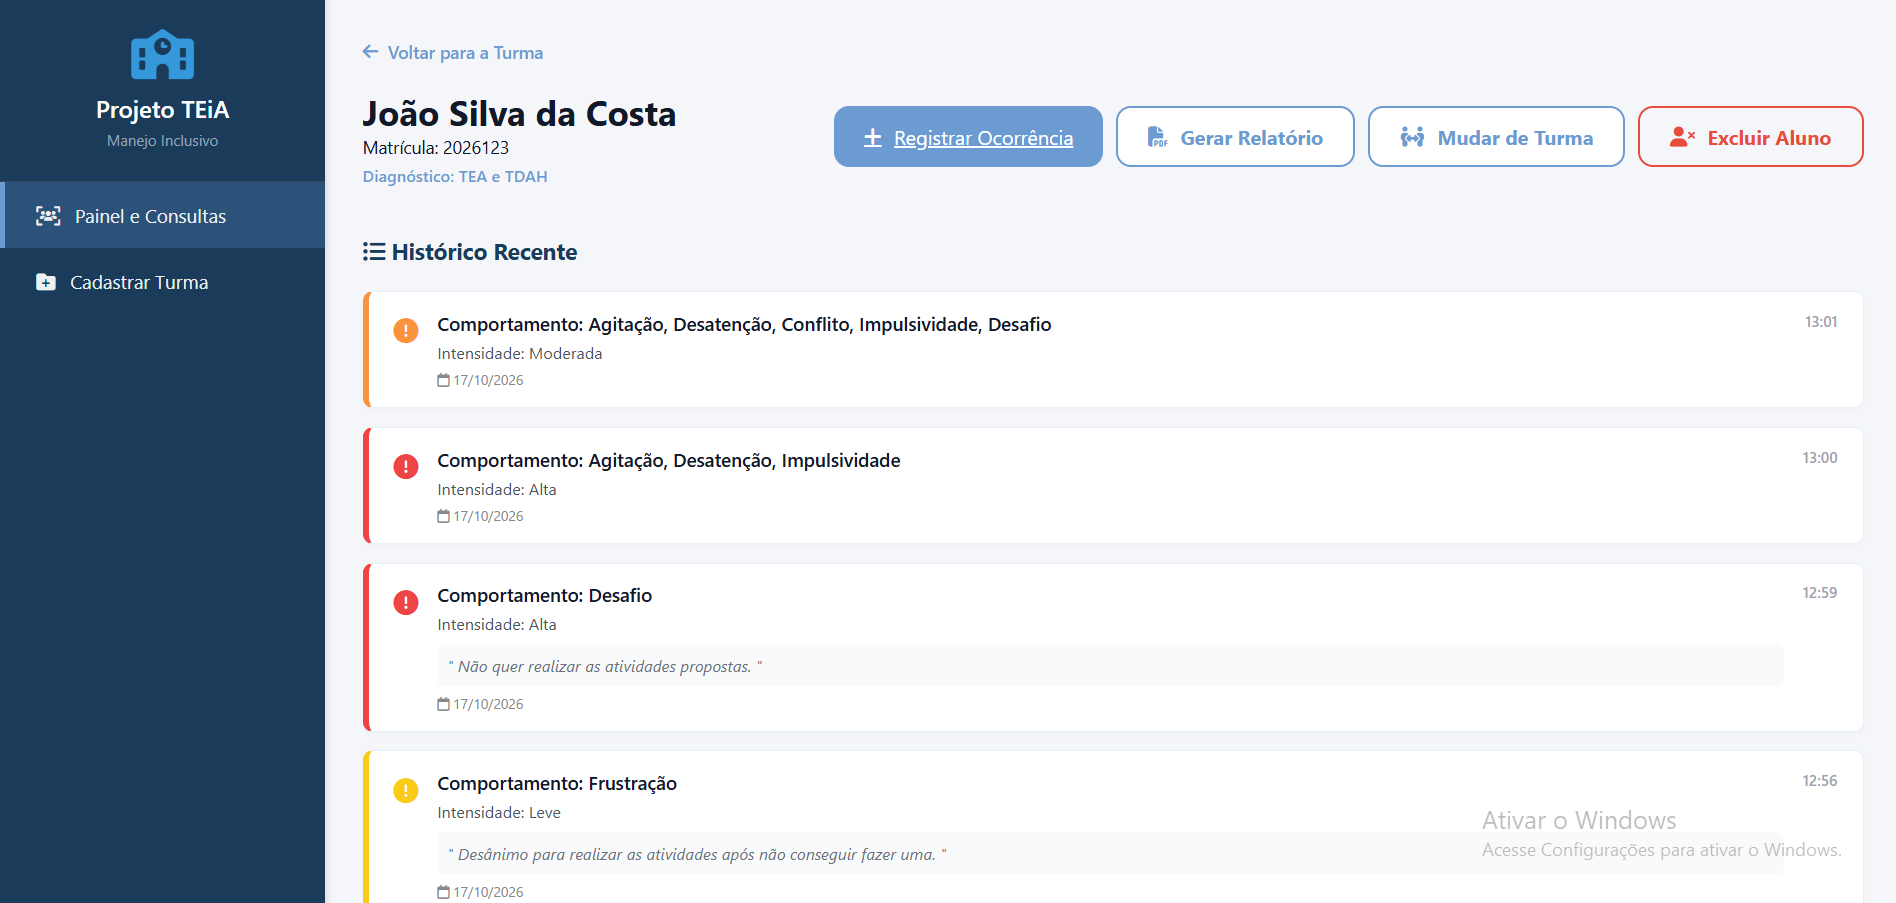
\includegraphics[width=\textwidth, keepaspectratio]
    {assets/painelAluno_desktop}
    \vspace{0.1cm}
    \centerline{\small (a) Desktop} % <-- Subtítulo A
  \end{minipage}\hfill
  \begin{minipage}[b]{0.22\textwidth}
    \centering
    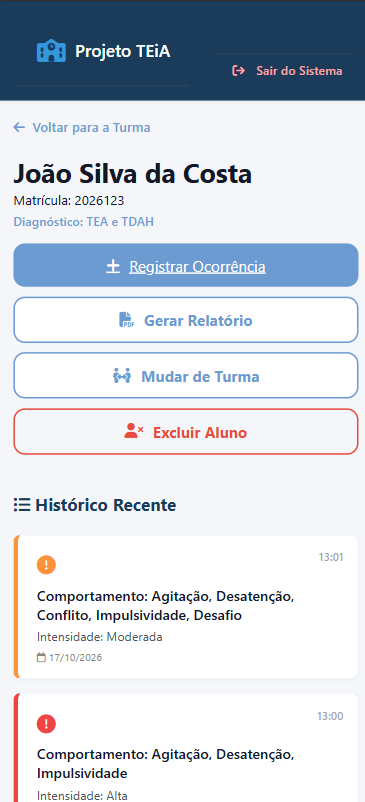
\includegraphics[width=\textwidth, keepaspectratio]
    {assets/painelAluno_mobile}
    \vspace{0.1cm}
        \centerline{\small (b) Mobile}
  \end{minipage}

  \vspace{0.3cm}
  \begin{flushleft}
  \footnotesize{Fonte: Elaborada pela autora (2026).}
  \end{flushleft}
\end{figure}

\vspace{0.5cm}
\subsection{Emissão de Relatórios para Apoio Clínico}

A Figura 5.7 ilustra a funcionalidade de geração de relatórios, acionada por meio do botão "Gerar Relatório" presente no perfil do estudante. O atendimento adequado de alunos com neurodivergências exige a partilha de informações consolidadas com a rede de apoio externa, que inclui profissionais de saúde (neuropediatras, psicólogos ou terapeutas). Para suprir esta necessidade, estipulada no Requisito Funcional RF07, o sistema TEia foi dotado de uma funcionalidade de exportação automatizada.

O \textit{software} compila o cabeçalho de identificação do aluno (nome, matrícula e diagnóstico clínico) e toda a cronologia do seu "Histórico Recente", formatando a página para impressão de maneira limpa e isenta de elementos de navegação (como os menus laterais). A janela de diálogo nativa do navegador é então acionada, permitindo ao educador ou ao gestor escolar guardar o documento diretamente em formato PDF. Este fluxo não apenas digitaliza o processo do diário de classe, mas transforma os registros isolados do professor em um dossiê clínico-pedagógico pronto a ser anexado ao prontuário médico do aluno.

\begin{figure}[H]
    \centering
    \caption{Tela Emissão de Relatórios para Apoio Clínico}
    \label{fig:EmissãoRelatóriosApoioClínico}
    
    \vspace{0.2cm}
    
   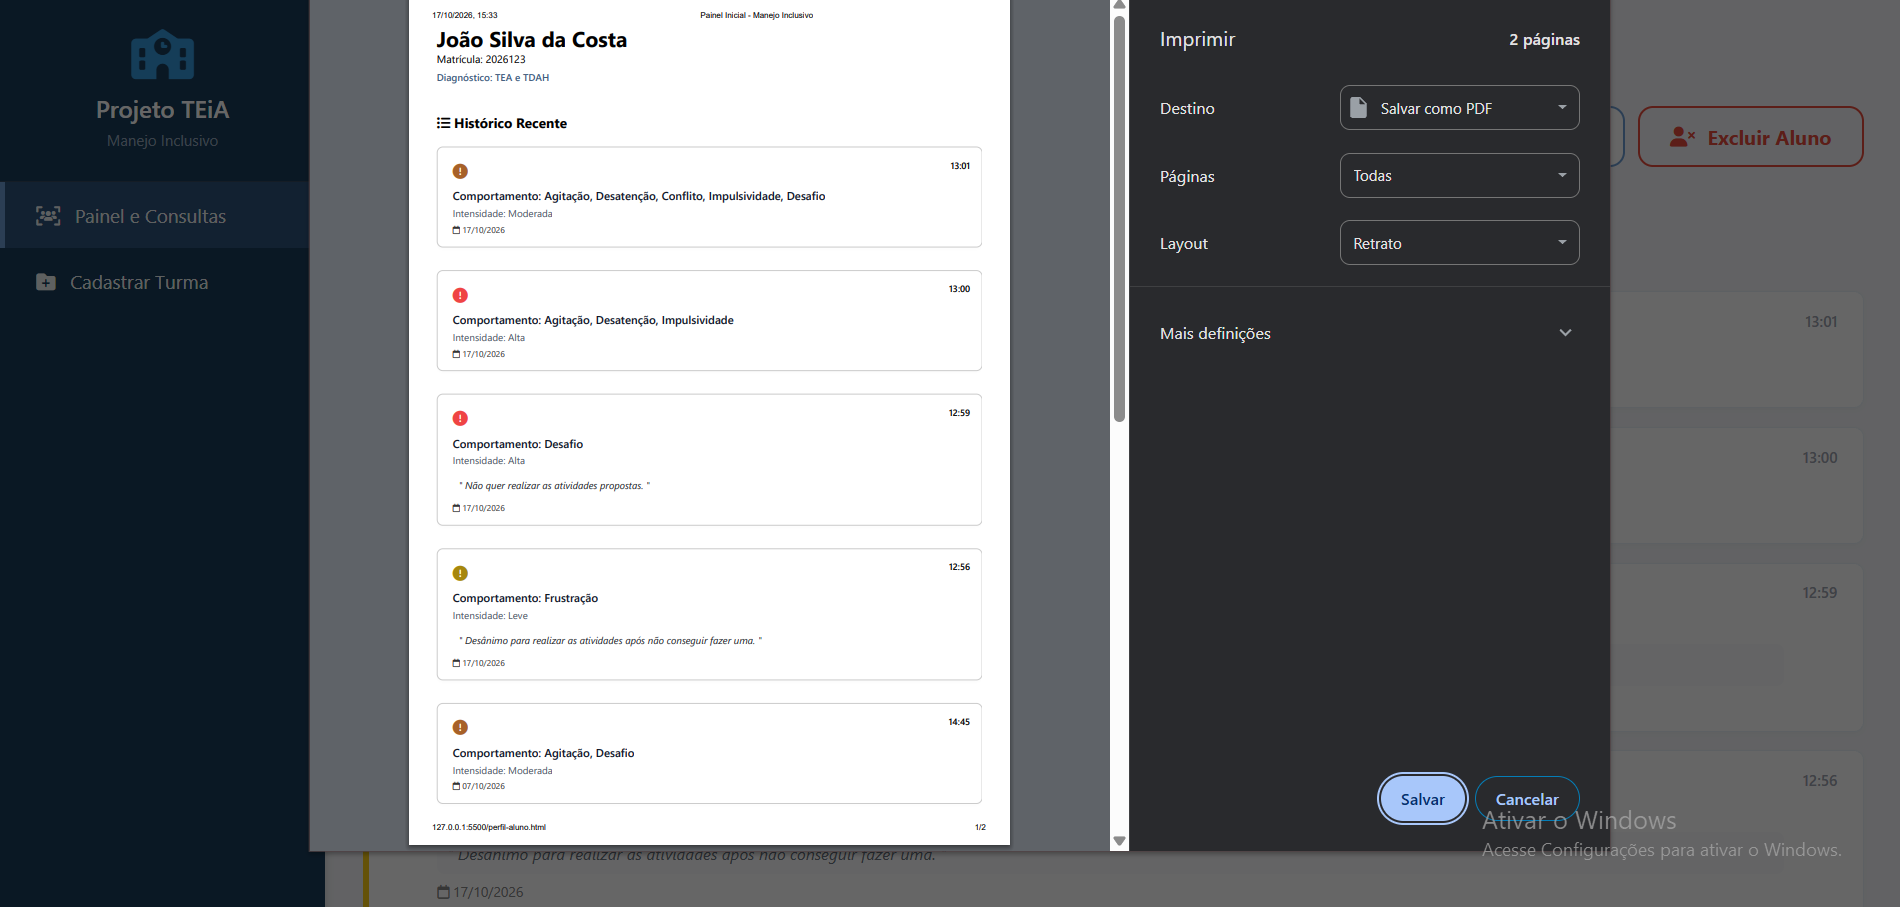
\includegraphics[width=0.8\textwidth, keepaspectratio]{assets/relatorio}
    
    \vspace{0.2cm}
    
    \begin{flushleft}
        \footnotesize Fonte: Elaborada pela autora (2026).
    \end{flushleft}
\end{figure}

\vspace{0.5cm}
\subsection{Registro Ágil de Ocorrências}

A Figura 5.8 exibe o modal de "Novo Registro", que é acionado pelo educador diretamente a partir do perfil do aluno. O \textit{design} desta interface foi concebido com foco na otimização do tempo em sala de aula, sendo este um requisito não funcional crítico (RNF02) para evitar a interrupção da dinâmica letiva durante o manejo de uma crise.

Para alcançar essa agilidade técnica e cognitiva, a aplicação minimizou a dependência de campos textuais livres. O tradicional formulário de digitação foi substituído por botões de seleção rápida (\textit{chips} interativos) construídos com CSS e \textit{Vanilla JS}. O professor apenas clica para categorizar os múltiplos "Comportamentos Observados" simultâneos (como exemplificado na imagem pelas marcações em Agitação, Desatenção, Conflito, Impulsividade e Desafio) e definir o nível de "Intensidade" do evento (Leve, Moderada ou Alta). 

Embora o sistema encoraje a seleção rápida, o campo para "Observações" textuais foi mantido opcionalmente, permitindo ao professor, caso tenha tempo hábil, detalhar o contexto do evento (ex: "Apresentou um nível de agitação muito elevado e desatenção severa..."). Esta abordagem de usabilidade garante um registro robusto que alimentará o banco de dados. O botão de submissão ("Salvar e Ver Sugestões") evidencia a premissa principal do sistema TEia: a transição imediata do registro passivo para a oferta de suporte pedagógico proativo.

\begin{figure}[H]
  \centering
  \caption{Tela de Registro Ágil de Ocorrências}
  \label{fig:tela_registroOcorrencia}
  \vspace{0.3cm}

  \begin{minipage}[b]{0.77\textwidth}
    \centering
    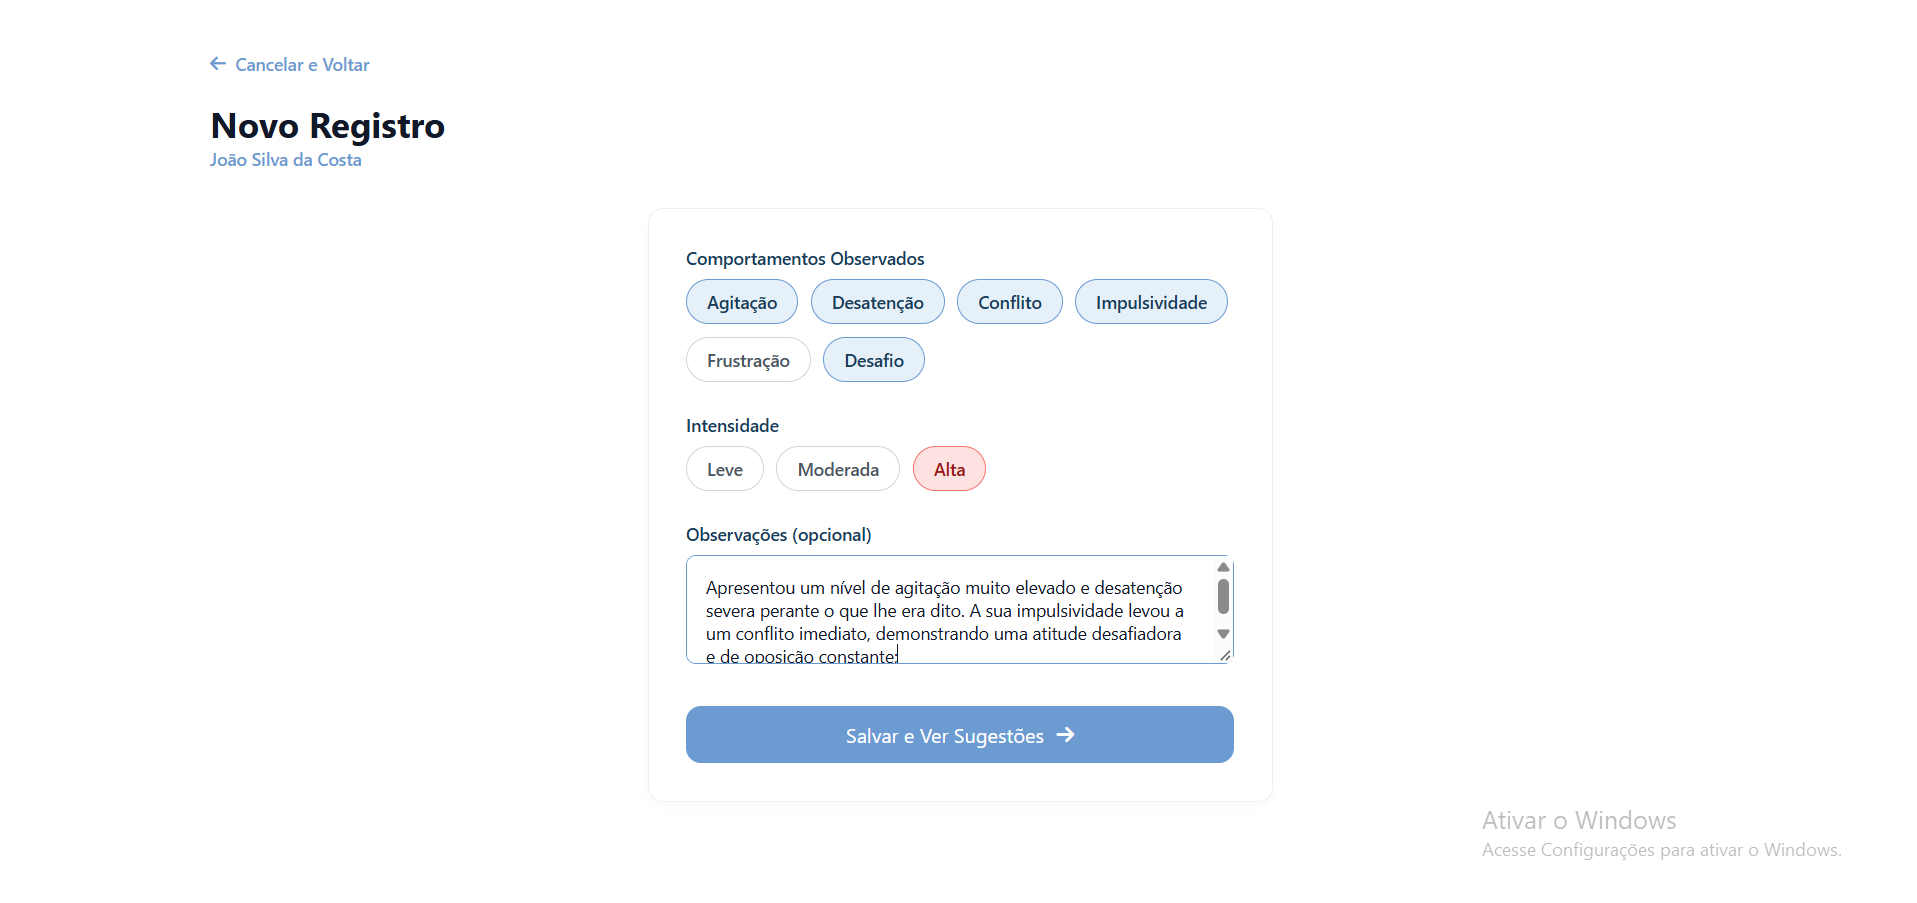
\includegraphics[width=\textwidth, keepaspectratio]
    {assets/registroOcorrencia_desktop}
    \vspace{0.1cm}
    \centerline{\small (a) Desktop} % <-- Subtítulo A
  \end{minipage}\hfill
  \begin{minipage}[b]{0.22\textwidth}
    \centering
    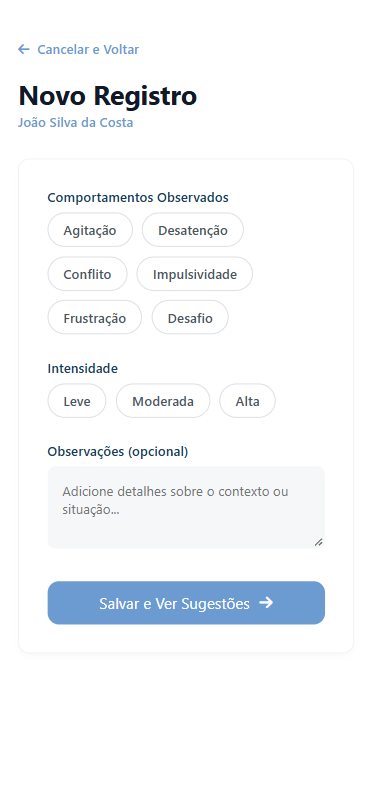
\includegraphics[width=\textwidth, keepaspectratio]
    {assets/registroOcorrencia_mobile}
    \vspace{0.1cm}
        \centerline{\small (b) Mobile}
  \end{minipage}

  \vspace{0.3cm}
  \begin{flushleft}
  \footnotesize{Fonte: Elaborada pela autora (2026).}
  \end{flushleft}
\end{figure}

\vspace{0.5cm}
\subsection{Sugestão de Manejo Comportamental}

A Figura 5.9 exibe a interface de "Sugestões de Manejo", que constitui a entrega de valor pedagógico central da plataforma TEia. Imediatamente após a submissão de um registro de ocorrência, a lógica do \textit{front-end} processa as informações inseridas e direciona o educador para esta tela, que atua como um assistente comportamental dinâmico.

Em vez de apenas armazenar o dado passivamente no banco de dados, o sistema apresenta um conjunto de \textit{cards} com design claro (fundo verde pastel) e ícones ilustrativos, sugerindo intervenções educacionais e clínicas fundamentadas em evidências para o comportamento recém-registrado. Como exemplificado na interface, as estratégias sugeridas incluem táticas de autorregulação (ex: "Pausa para Movimento"), adaptação da comunicação ("Instruções Curtas"), previsibilidade ("Ambiente Estruturado") e suporte emocional ("Reforço Positivo").

A coerência visual e o texto direto permitem que o professor assimile as orientações em questão de segundos, promovendo a estabilização do aluno durante uma crise. Após a leitura e aplicação da estratégia, o docente confirma a ação por meio do botão central ("Entendi"), o que o redireciona de volta ao painel da turma para dar continuidade à rotina letiva.

\begin{figure}[H]
  \centering
  \caption{Tela de Sugestão de Manejo Comportamental}
  \label{fig:tela_registroOcorrencia}
  \vspace{0.3cm}

  \begin{minipage}[b]{0.77\textwidth}
    \centering
    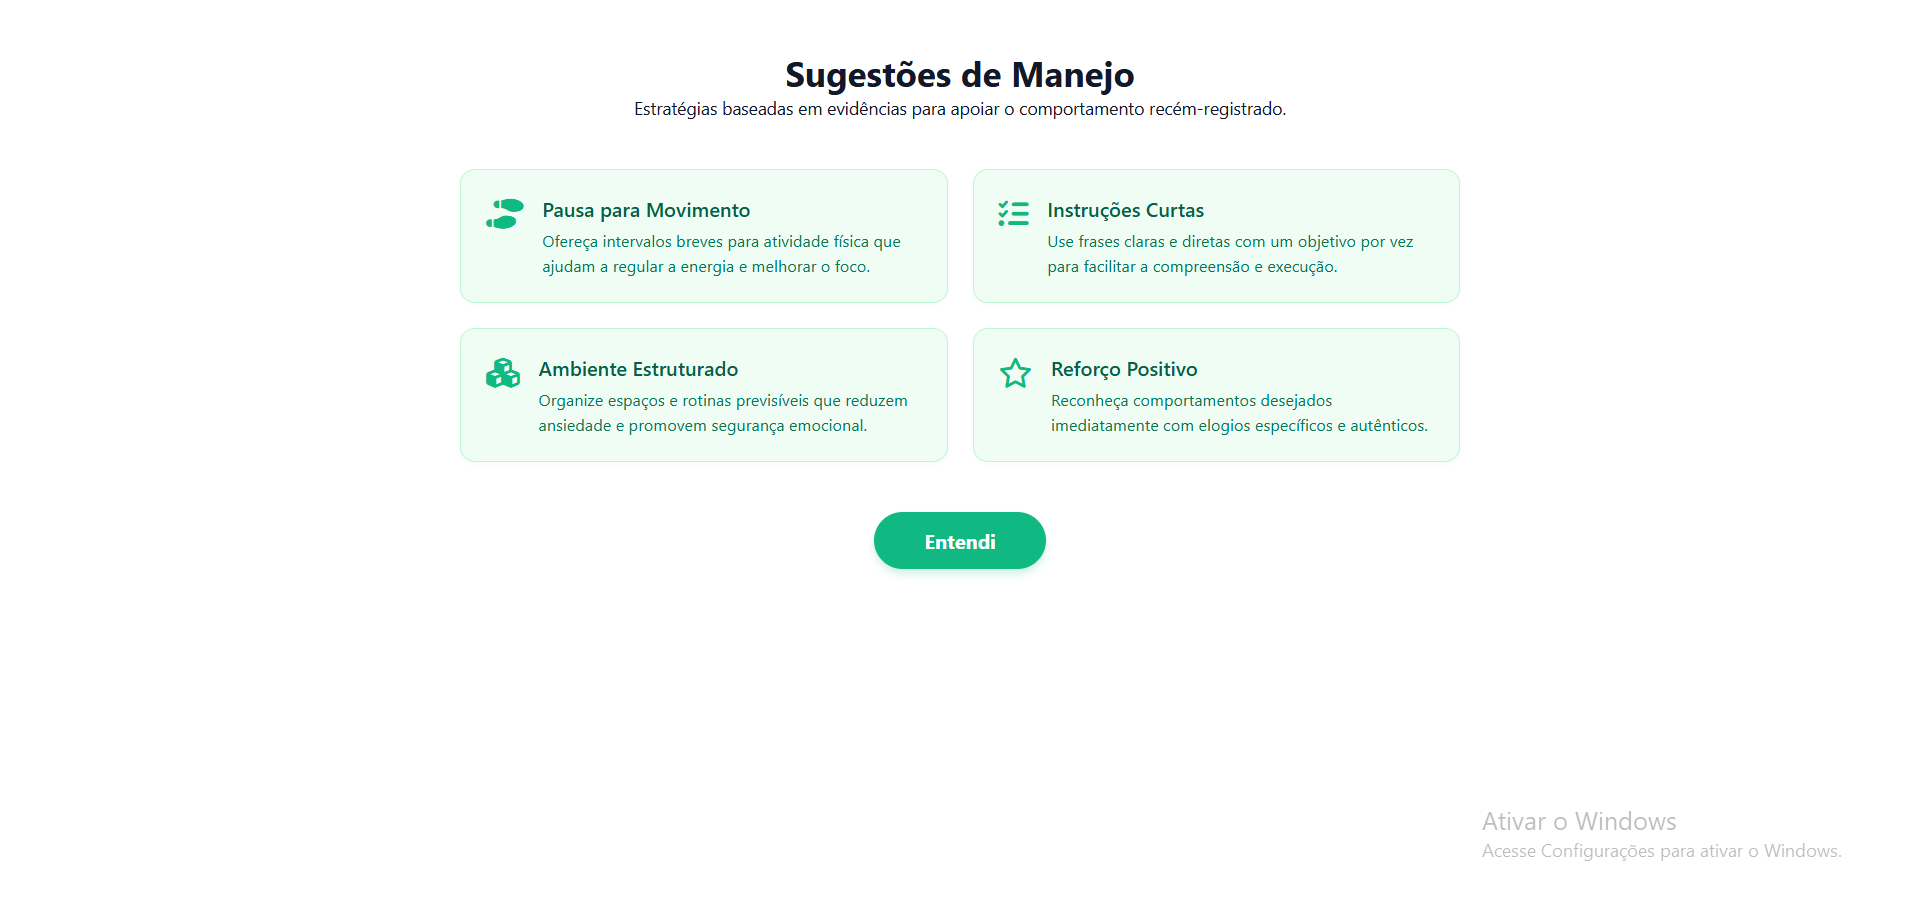
\includegraphics[width=\textwidth, keepaspectratio]
    {assets/SugestãoManejo_desktop}
    \vspace{0.1cm}
    \centerline{\small (a) Desktop} % <-- Subtítulo A
  \end{minipage}\hfill
  \begin{minipage}[b]{0.22\textwidth}
    \centering
    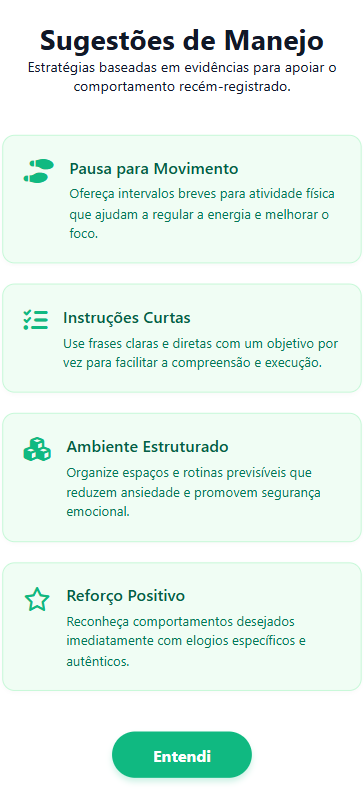
\includegraphics[width=\textwidth, keepaspectratio]
    {assets/SugestãoManejo_mobile}
    \vspace{0.1cm}
        \centerline{\small (b) Mobile}
  \end{minipage}

  \vspace{0.3cm}
  \begin{flushleft}
  \footnotesize{Fonte: Elaborada pela autora (2026).}
  \end{flushleft}
\end{figure}

\vspace{0.5cm}
\section{Interfaces do Perfil Gestão Escolar}

O perfil de Gestão Escolar foi estruturado no sistema TEia sob o princípio de \textit{Role-Based Access Control} (RBAC). Ele atua exclusivamente na supervisão institucional, possuindo amplos privilégios de "somente leitura" aliados a rigorosas travas de segurança (\textit{UI/UX}) que ocultam comandos de edição. O objetivo dessa arquitetura é evitar a modificação indevida de dados, garantindo que o controle da chamada e a veracidade do prontuário comportamental permaneçam sob responsabilidade exclusiva dos educadores presentes em sala de aula.

\vspace{0.5cm}
\subsection{Motor de Busca e Visão Global da Gestão}

A Figura 5.10 ilustra a interface de "Visão Global da Gestão". Esta tela espelha o painel do educador, porém quebra as barreiras de isolamento de dados do professor, permitindo que a coordenação visualize o \textit{dashboard} central com todas as turmas ativas na instituição. 

O destaque é o módulo de "Busca Rápida e Filtros", que atua como ferramenta de rastreio dinâmico. Esta funcionalidade atende ao requisito de filtragem instantânea, permitindo à gestão localizar e pesquisar ativamente estudantes combinando múltiplos parâmetros simultâneos: Nome do Aluno, Turma, tipo de Neurodivergência e recortes de Período temporal.

\begin{figure}[H]
  \centering
  \caption{Tela de Motor de Busca e Visão Global da Gestão}
  \label{fig:tela_visaoGlobal}
  \vspace{0.3cm}

  \begin{minipage}[b]{0.77\textwidth}
    \centering
    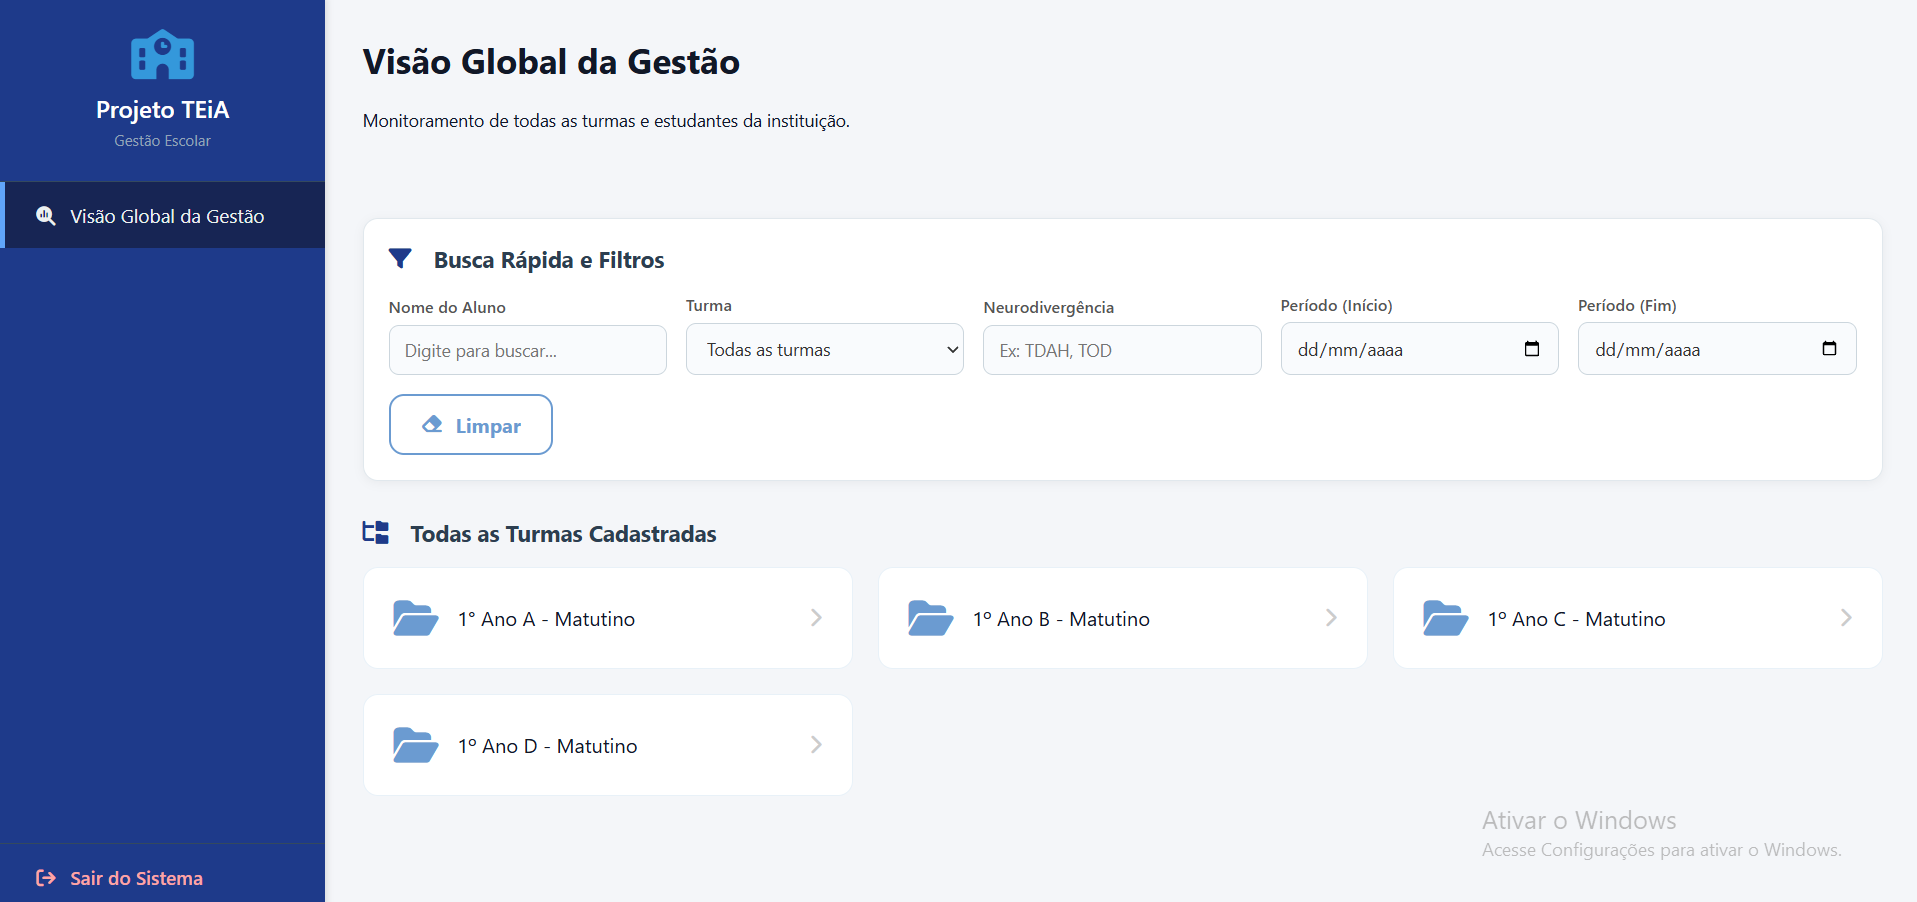
\includegraphics[width=\textwidth, keepaspectratio]
    {assets/visaoGlobal_desktop}
    \vspace{0.1cm}
    \centerline{\small (a) Desktop} % <-- Subtítulo A
  \end{minipage}\hfill
  \begin{minipage}[b]{0.22\textwidth}
    \centering
    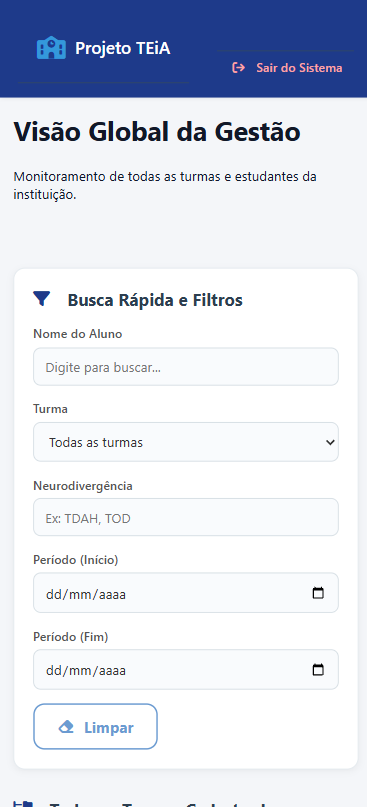
\includegraphics[width=\textwidth, keepaspectratio]
    {assets/visaoGlobal_mobile}
    \vspace{0.1cm}
        \centerline{\small (b) Mobile}
  \end{minipage}

  \vspace{0.3cm}
  \begin{flushleft}
  \footnotesize{Fonte: Elaborada pela autora (2026).}
  \end{flushleft}
\end{figure}

\vspace{0.5cm}
\subsection{Acesso Restrito ao Histórico e Emissão de Relatórios}

A partir do painel irrestrito, a gestão pode acessar qualquer turma para consultar a lista de estudantes, conforme demonstrado na Figura 5.11. É possível notar a efetividade das travas de segurança: os botões que alteram o estado do sistema (\textit{state mutation}), como "Novo Aluno" e "Excluir Turma", foram dinamicamente removidos da \textit{interface}, garantindo que o quadro de chamada seja gerido estritamente pelo educador responsável.

\begin{figure}[H]
  \centering
  \caption{Tela de Visão do Aluno pelo Gestor}
  \label{fig:tela_visaoGlobal}
  \vspace{0.3cm}

  \begin{minipage}[b]{0.77\textwidth}
    \centering
    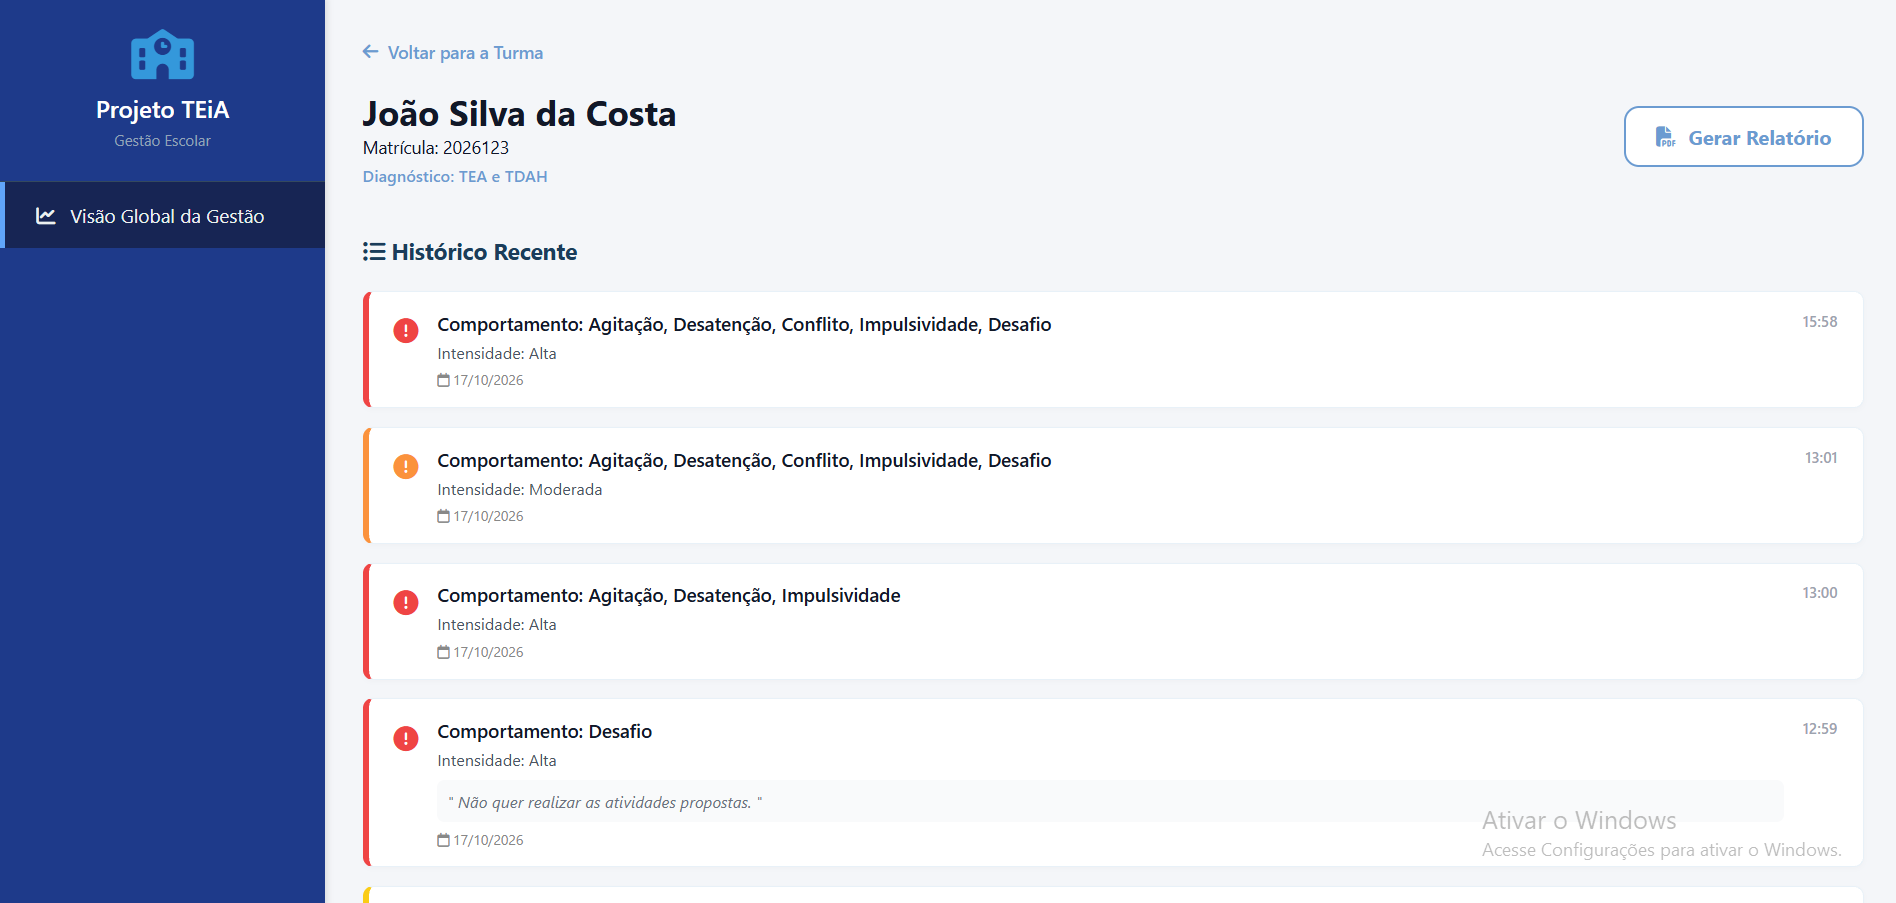
\includegraphics[width=\textwidth, keepaspectratio]
    {assets/acessoRestrito_desktop}
    \vspace{0.1cm}
    \centerline{\small (a) Desktop} % <-- Subtítulo A
  \end{minipage}\hfill
  \begin{minipage}[b]{0.22\textwidth}
    \centering
    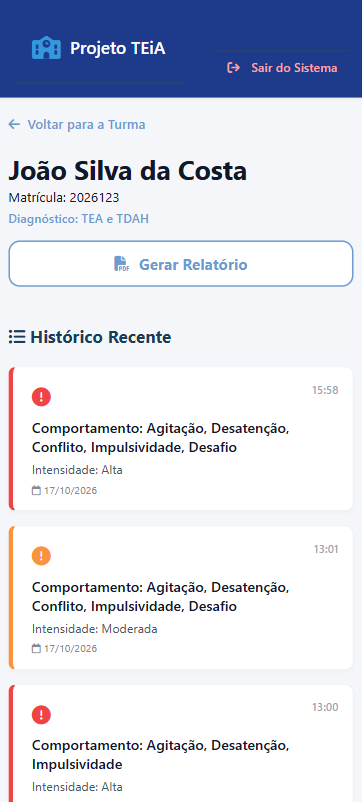
\includegraphics[width=\textwidth, keepaspectratio]
    {assets/acessoRestrito_mobile}
    \vspace{0.1cm}
        \centerline{\small (b) Mobile}
  \end{minipage}

  \vspace{0.3cm}
  \begin{flushleft}
  \footnotesize{Fonte: Elaborada pela autora (2026).}
  \end{flushleft}
\end{figure}

\vspace{0.5cm}
\section{Interfaces do Perfil Familiar}

O perfil Familiar foi idealizado para democratizar a informação, proporcionando uma comunicação contínua entre a escola e a rede de apoio domiciliar do aluno neurodivergente.

\vspace{0.5cm}
\subsection{Acompanhamento Transparente: Linha do Tempo (\textit{Timeline})}

A Figura 5.12 ilustra o painel de acesso exclusivo aos pais e responsáveis. Em oposição ao painel de gestão utilizado pelos professores, esta interface adota uma arquitetura em formato de linha do tempo (\textit{timeline}), desenhada com a abordagem \textit{Mobile-First}. Esse \textit{design} garante o acompanhamento da rotina escolar diretamente pelo celular com total mobilidade.

Os registros inseridos pelos professores no ambiente escolar são sincronizados em tempo real pelo banco de dados em nuvem e exibidos à família em \textit{cards} organizados cronologicamente. Para manter a coerência cognitiva em todo o sistema, a interface preserva a codificação semântica de cores de intensidade (como o laranja e o vermelho). Esta interface transparente soluciona a defasagem temporal característica dos "diários de papel", permitindo o alinhamento tempestivo das abordagens entre a escola e o ambiente doméstico.

\begin{figure}[H]
  \centering
  \caption{Tela de Acompanhamento Transparente: Linha do Tempo (\textit{Timeline})}
  \label{fig:tela_registroOcorrencia}
  \vspace{0.3cm}

  \begin{minipage}[b]{0.77\textwidth}
    \centering
    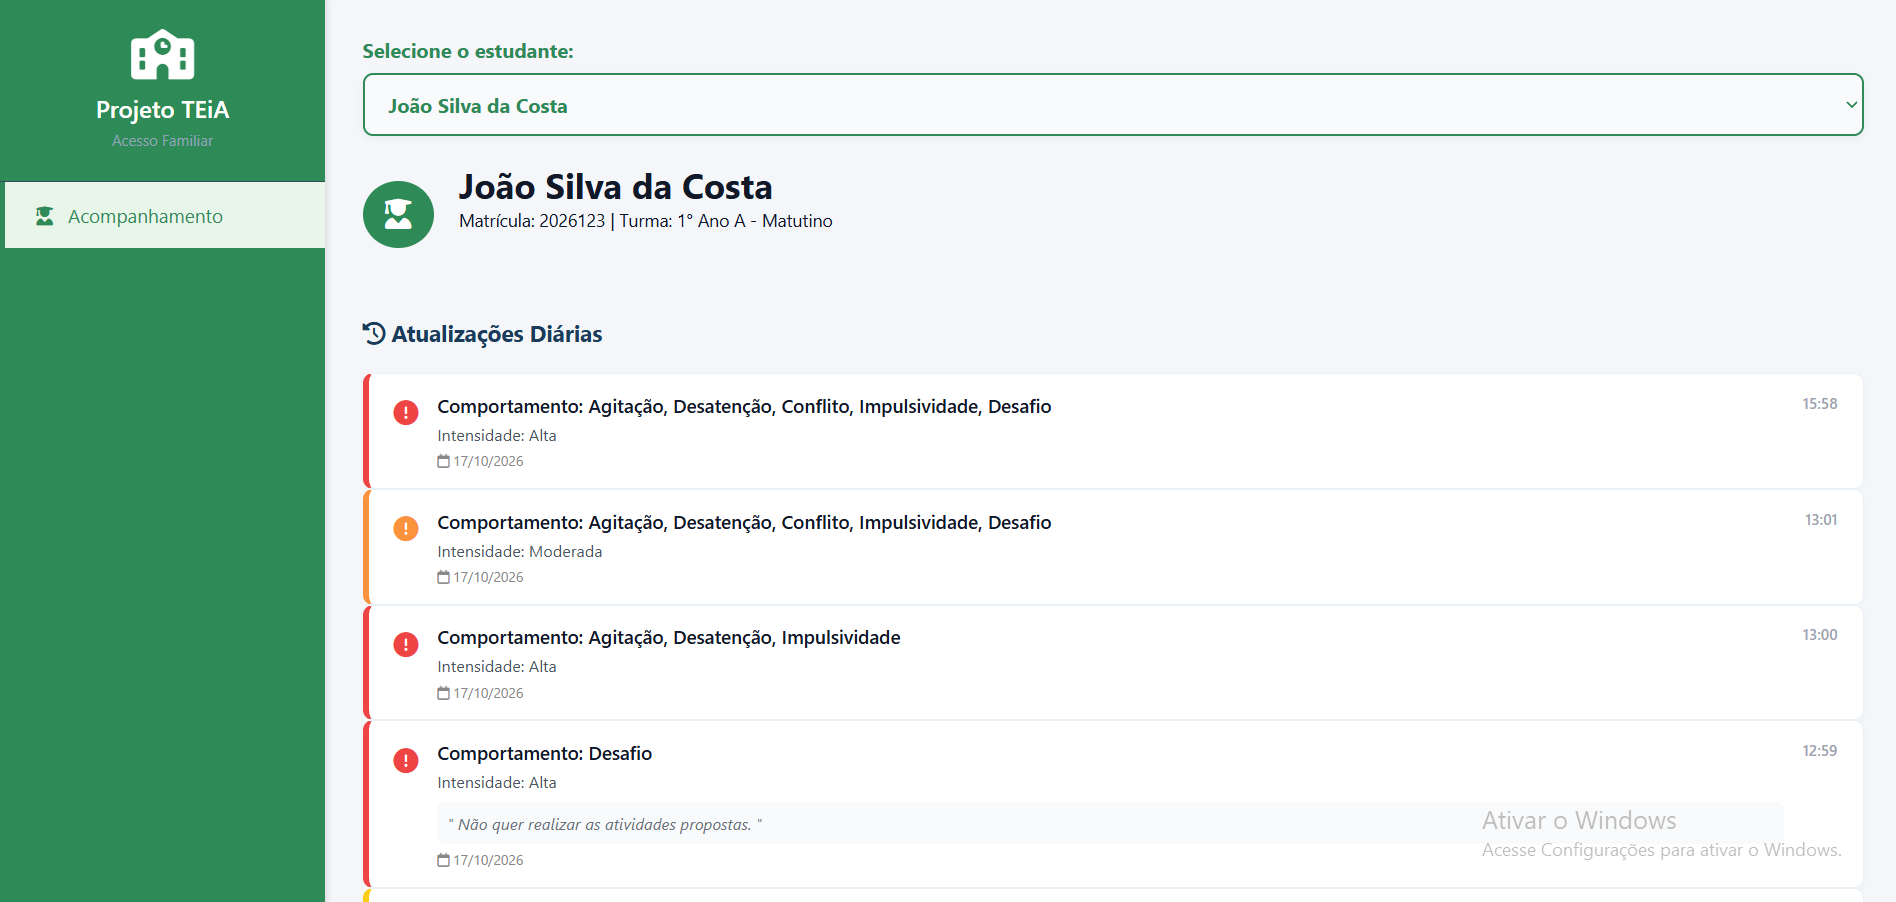
\includegraphics[width=\textwidth, keepaspectratio]
    {assets/timeline_desktop}
    \vspace{0.1cm}
    \centerline{\small (a) Desktop} % <-- Subtítulo A
  \end{minipage}\hfill
  \begin{minipage}[b]{0.22\textwidth}
    \centering
    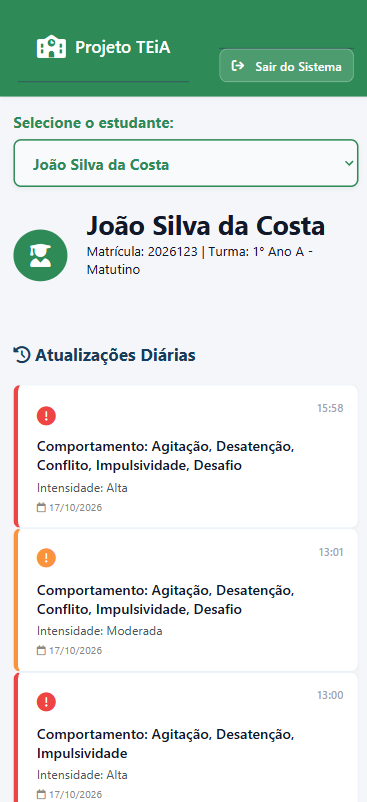
\includegraphics[width=\textwidth, keepaspectratio]
    {assets/timeline_mobile}
    \vspace{0.1cm}
        \centerline{\small (b) Mobile}
  \end{minipage}

  \vspace{0.3cm}
  \begin{flushleft}
  \footnotesize{Fonte: Elaborada pela autora (2026).}
  \end{flushleft}
\end{figure}